\documentclass{article}
\usepackage{ tipa }
\usepackage{amsfonts}
\usepackage{dsfont}
\usepackage{amssymb}
\usepackage{textcomp}
\usepackage{lmodern}
\usepackage[T1]{fontenc}
\usepackage[spanish,activeacute]{babel}
\usepackage{mathtools}
\usepackage{ mathrsfs }
\usepackage{booktabs}
\usepackage{multirow}
\usepackage{graphicx}
\usepackage{fancyhdr}
\usepackage{ dsfont }
\usepackage{ upgreek }
\usepackage{fancyhdr}
\usepackage{listings}
\pagestyle{fancy}
\lstset{language=Matlab, breaklines=true, basicstyle=\footnotesize}
\spanishdecimal{.}

\title{\includegraphics[scale=.5]{../../../Pictures/Ciencias.jpeg}\\\
Fundamentos de Android}
\author{Saavedra Rodrigo\\\
UNAM\\\
Tarea: Mi primer proyecto Android/2016-2}



\begin{document}
\maketitle
\pagenumbering{roman}

\fancyhead[L]{ Fundamentos de Android}
\fancyhead[R]{Tarea I, Saavedra Rodrigo}

\newpage

\noindent \textbf{Mi primer proyecto Android}:\\

\noindent \textbf{a)Idiomas}\\

$\alpha$. Espa\~{n}ol\

\begin{center}

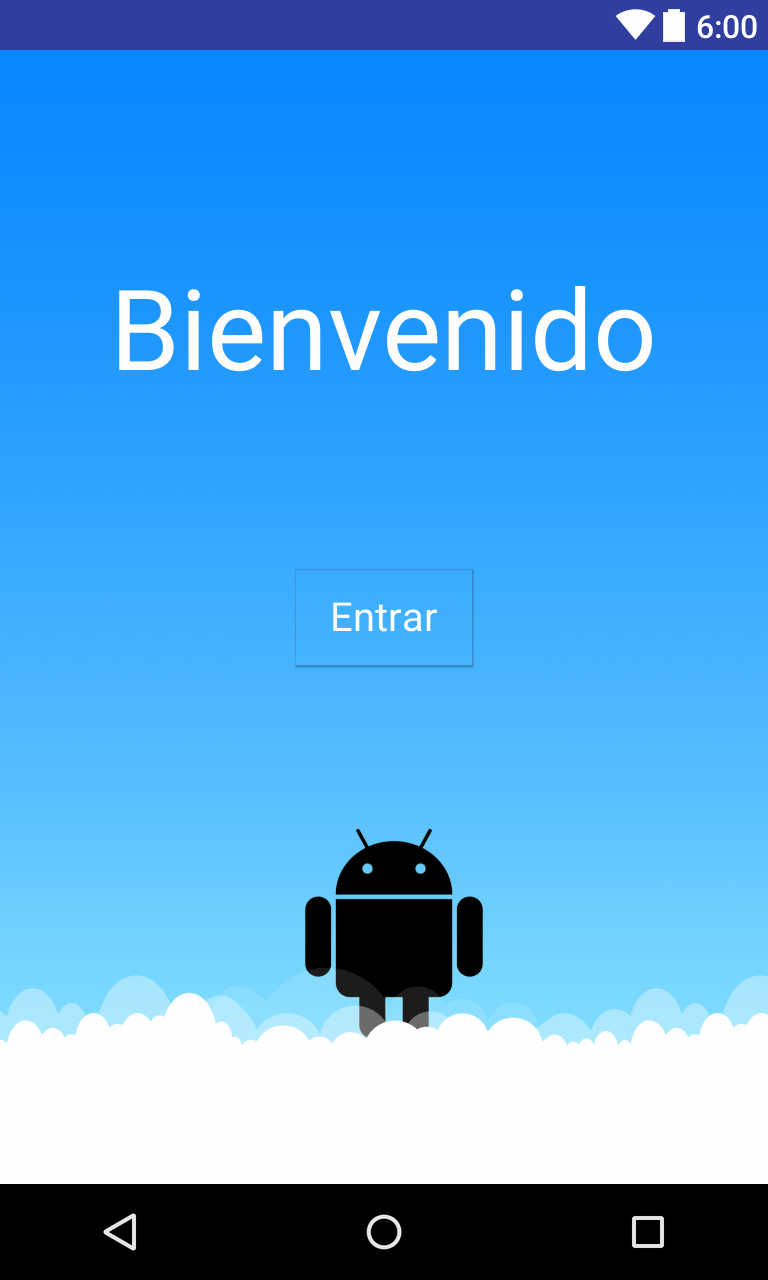
\includegraphics[scale=.15]{layout-2016-04-17-esp_lay.png} 

\end{center}

$\beta$. Ingl\'es\

\begin{center}

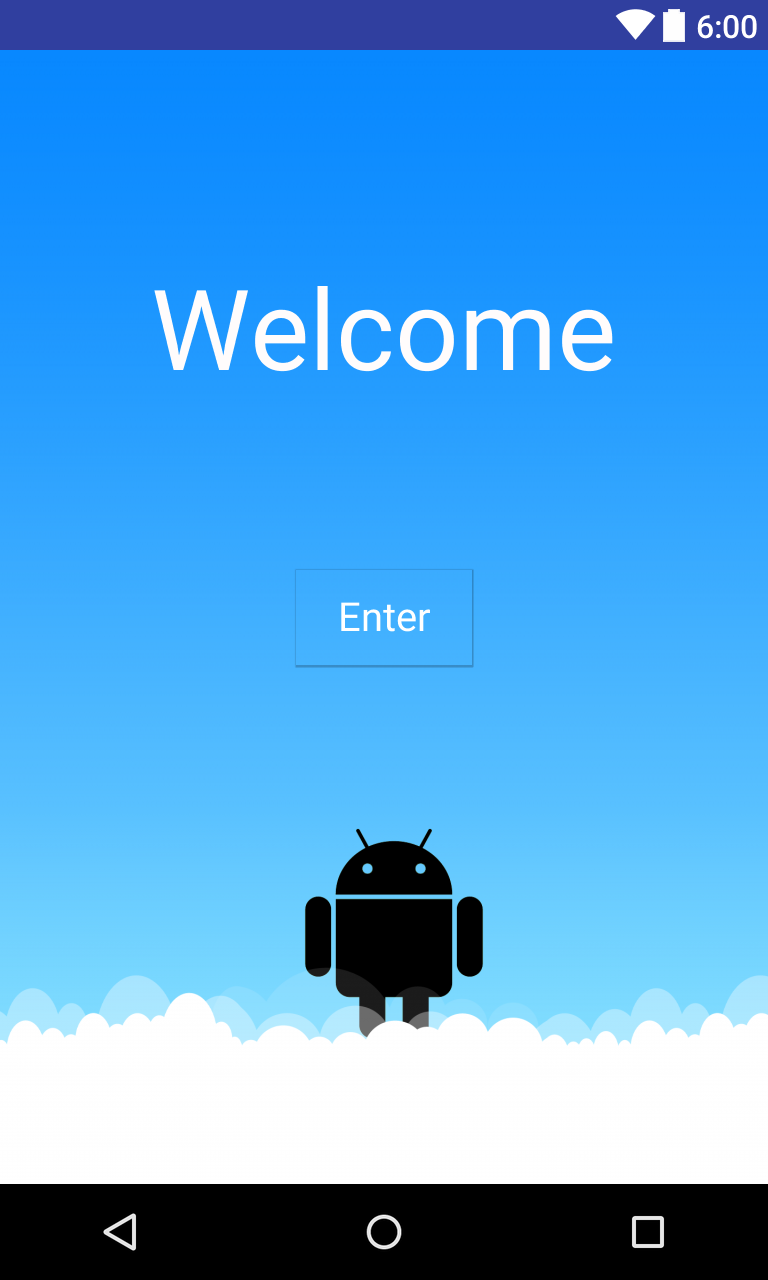
\includegraphics[scale=.15]{layout-2016-04-17-Eng_lay.png} 

\end{center}

\newpage

$\gamma$. Alem\'an\

\begin{center}

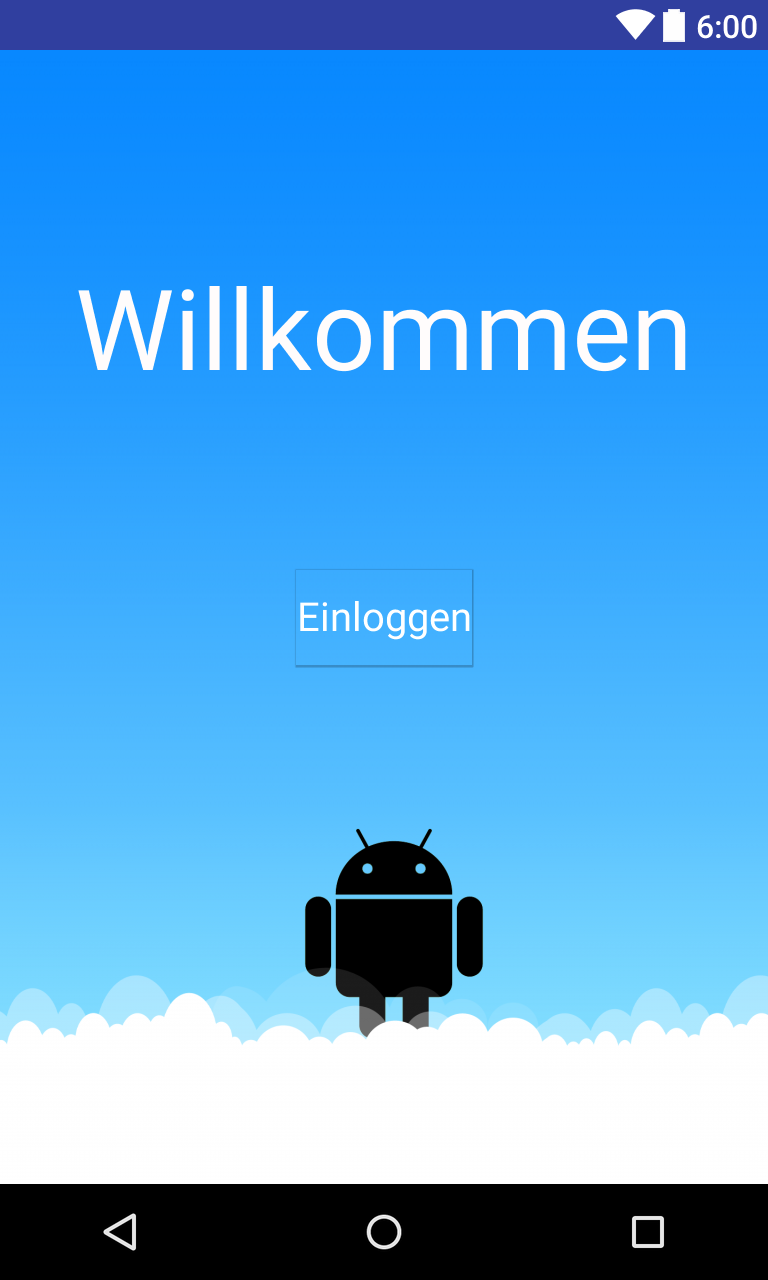
\includegraphics[scale=.15]{layout-2016-04-17-Deu_lay.png} 

\end{center}

$\delta$. Franc\'es\

\begin{center}

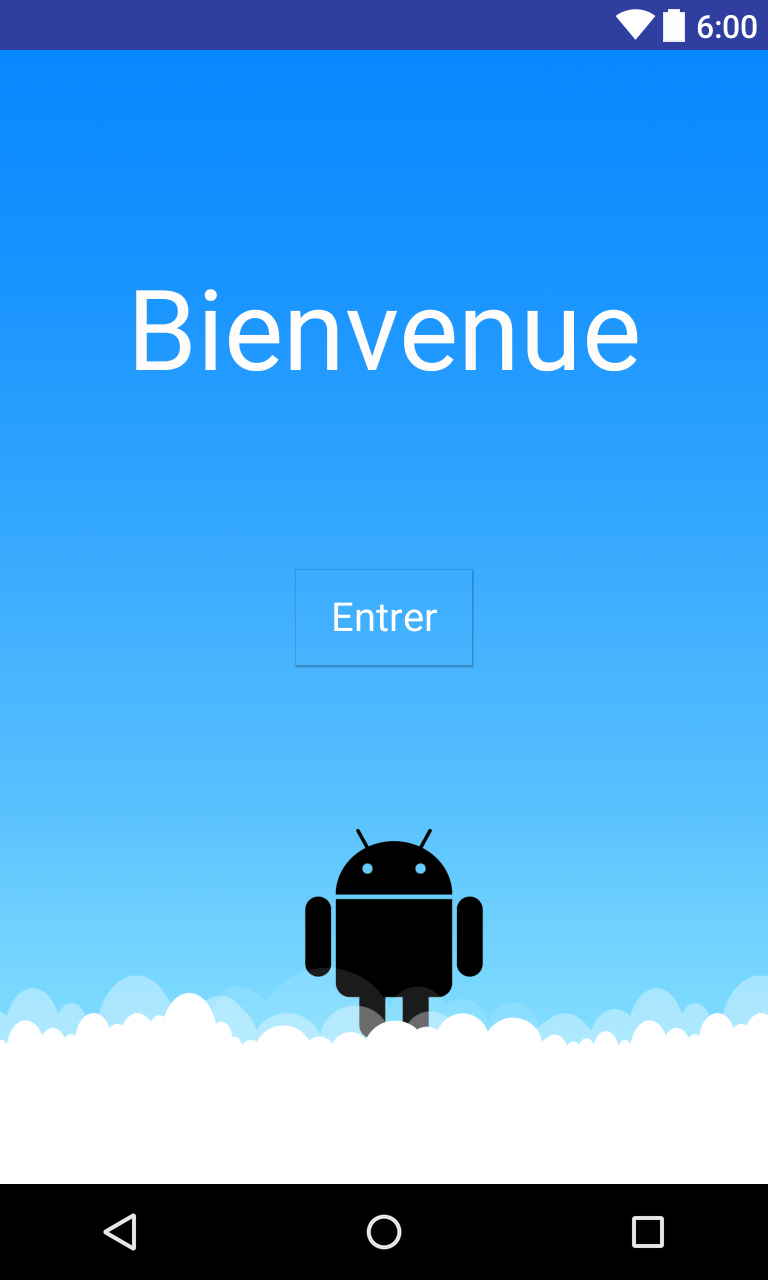
\includegraphics[scale=.15]{layout-2016-04-17-Fra_lay.png} 

\end{center}

\newpage

\noindent \textbf{b)Soporte tama\~{n}os de pantalla y orientaci\'on}\\

$\alpha$. Layout vertical\

\begin{center}

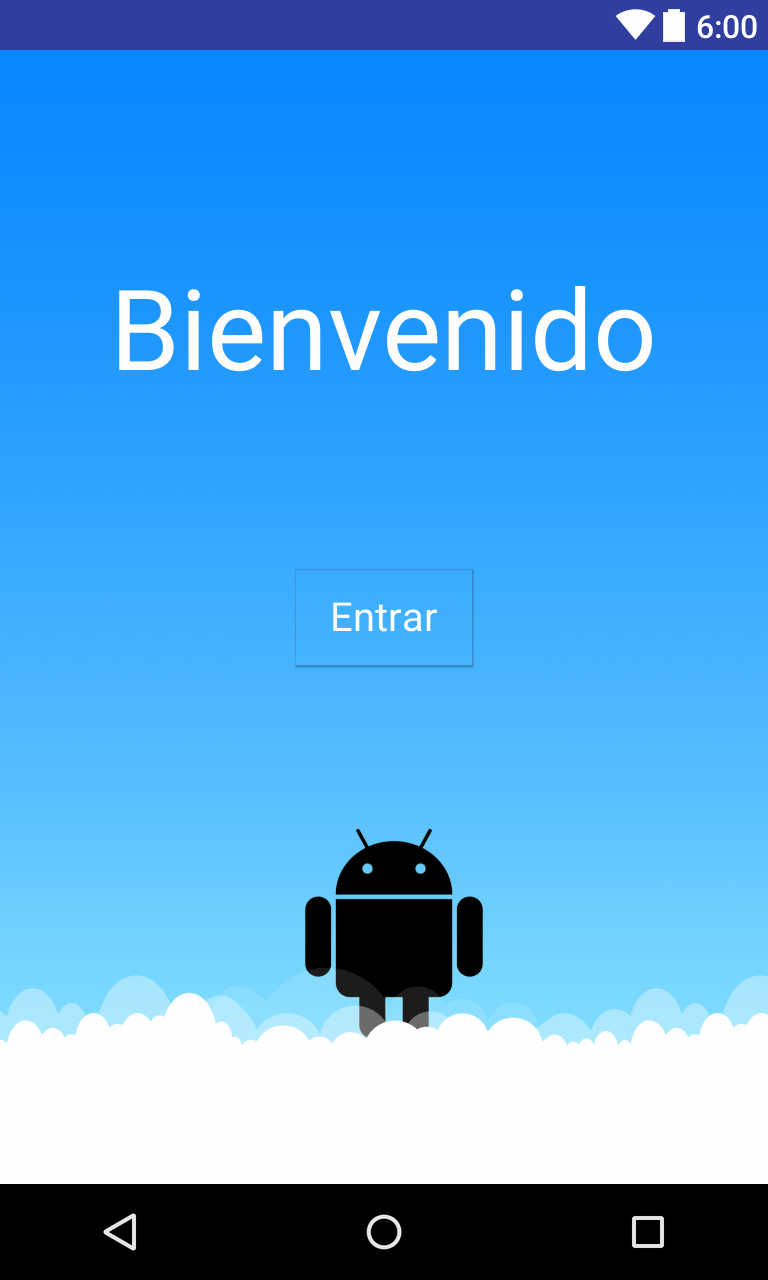
\includegraphics[scale=.15]{layout-2016-04-17-esp_lay.png} 

\end{center}

$\beta$. Layout Landscape\\\\\

\begin{center}

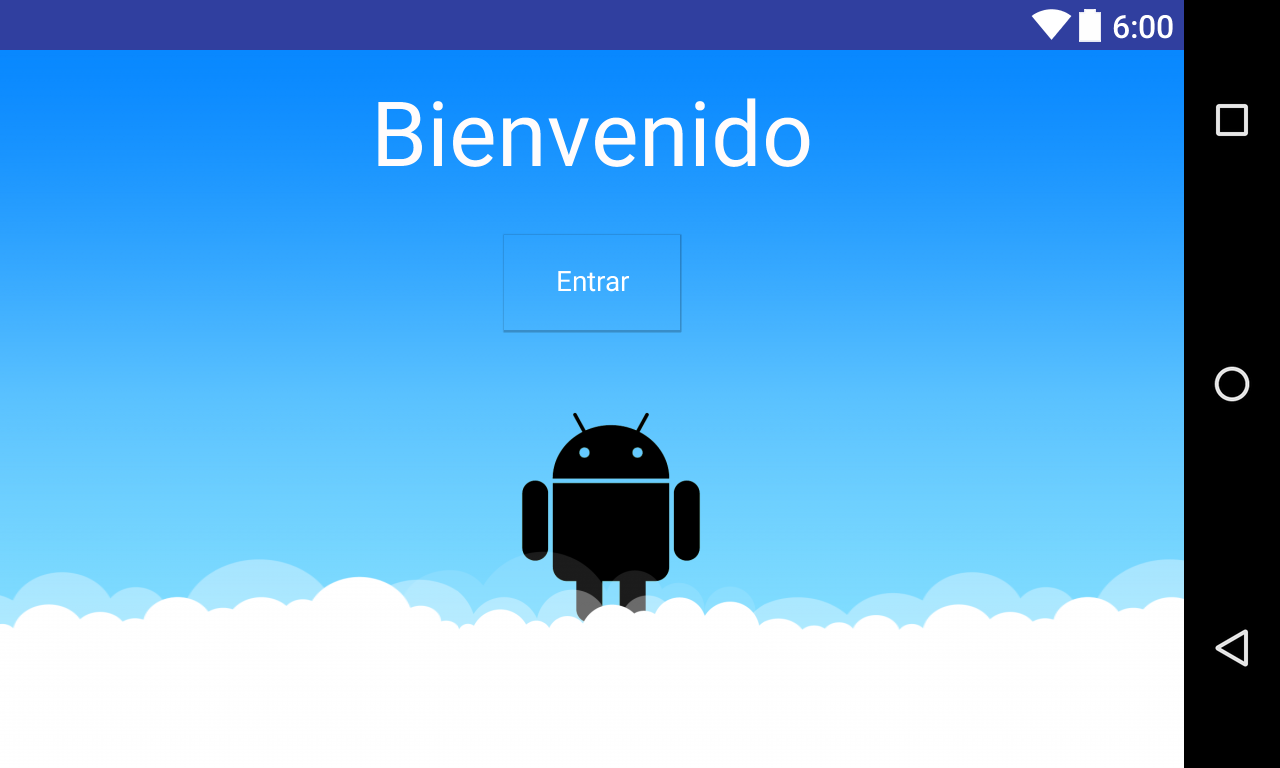
\includegraphics[scale=.15]{layout-2016-04-17-esp_layland.png} 

\end{center}

\newpage

$\gamma$. Layout Tableta vertical\

\begin{center}

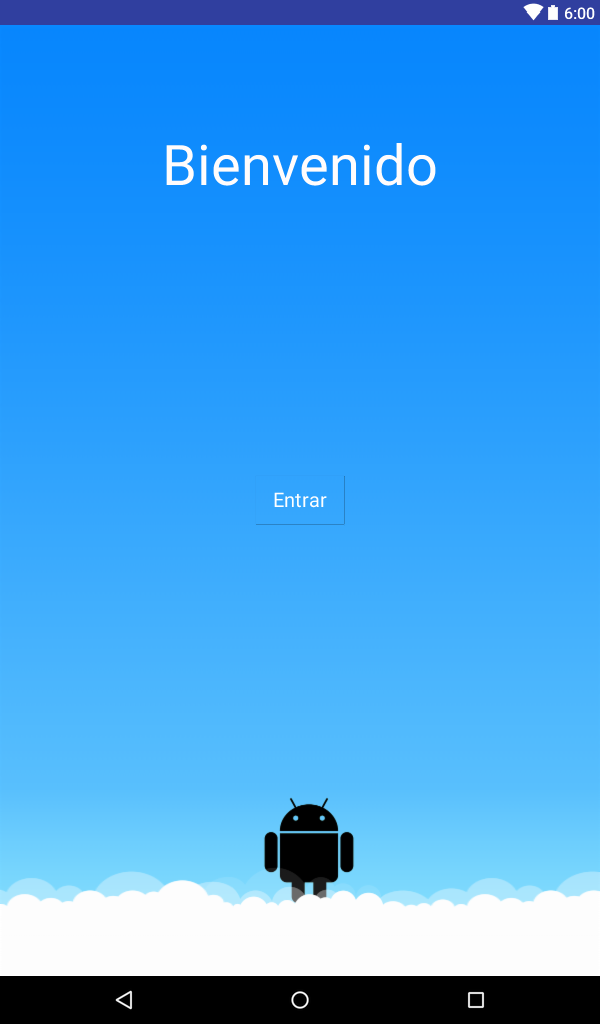
\includegraphics[scale=.2]{layout-2016-04-17-esp_tab_lay.png} 

\end{center}

$\delta$. Layout Tableta Landscape\\\\

\begin{center}

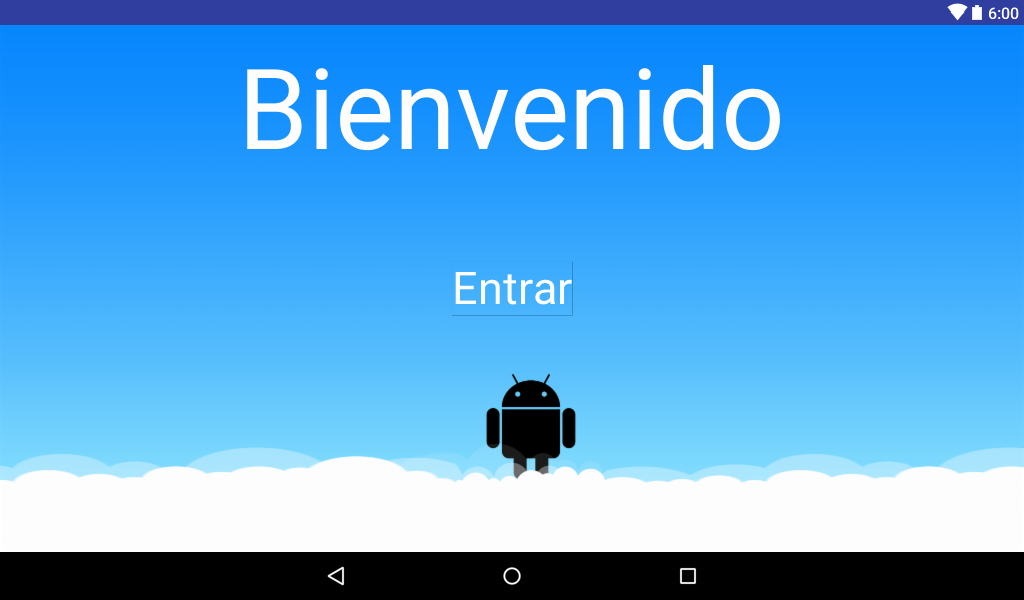
\includegraphics[scale=.25]{layout-2016-04-17-esp_tab_laylan.png} 

\end{center}

\newpage

$\epsilon$. Android TV

\begin{center}

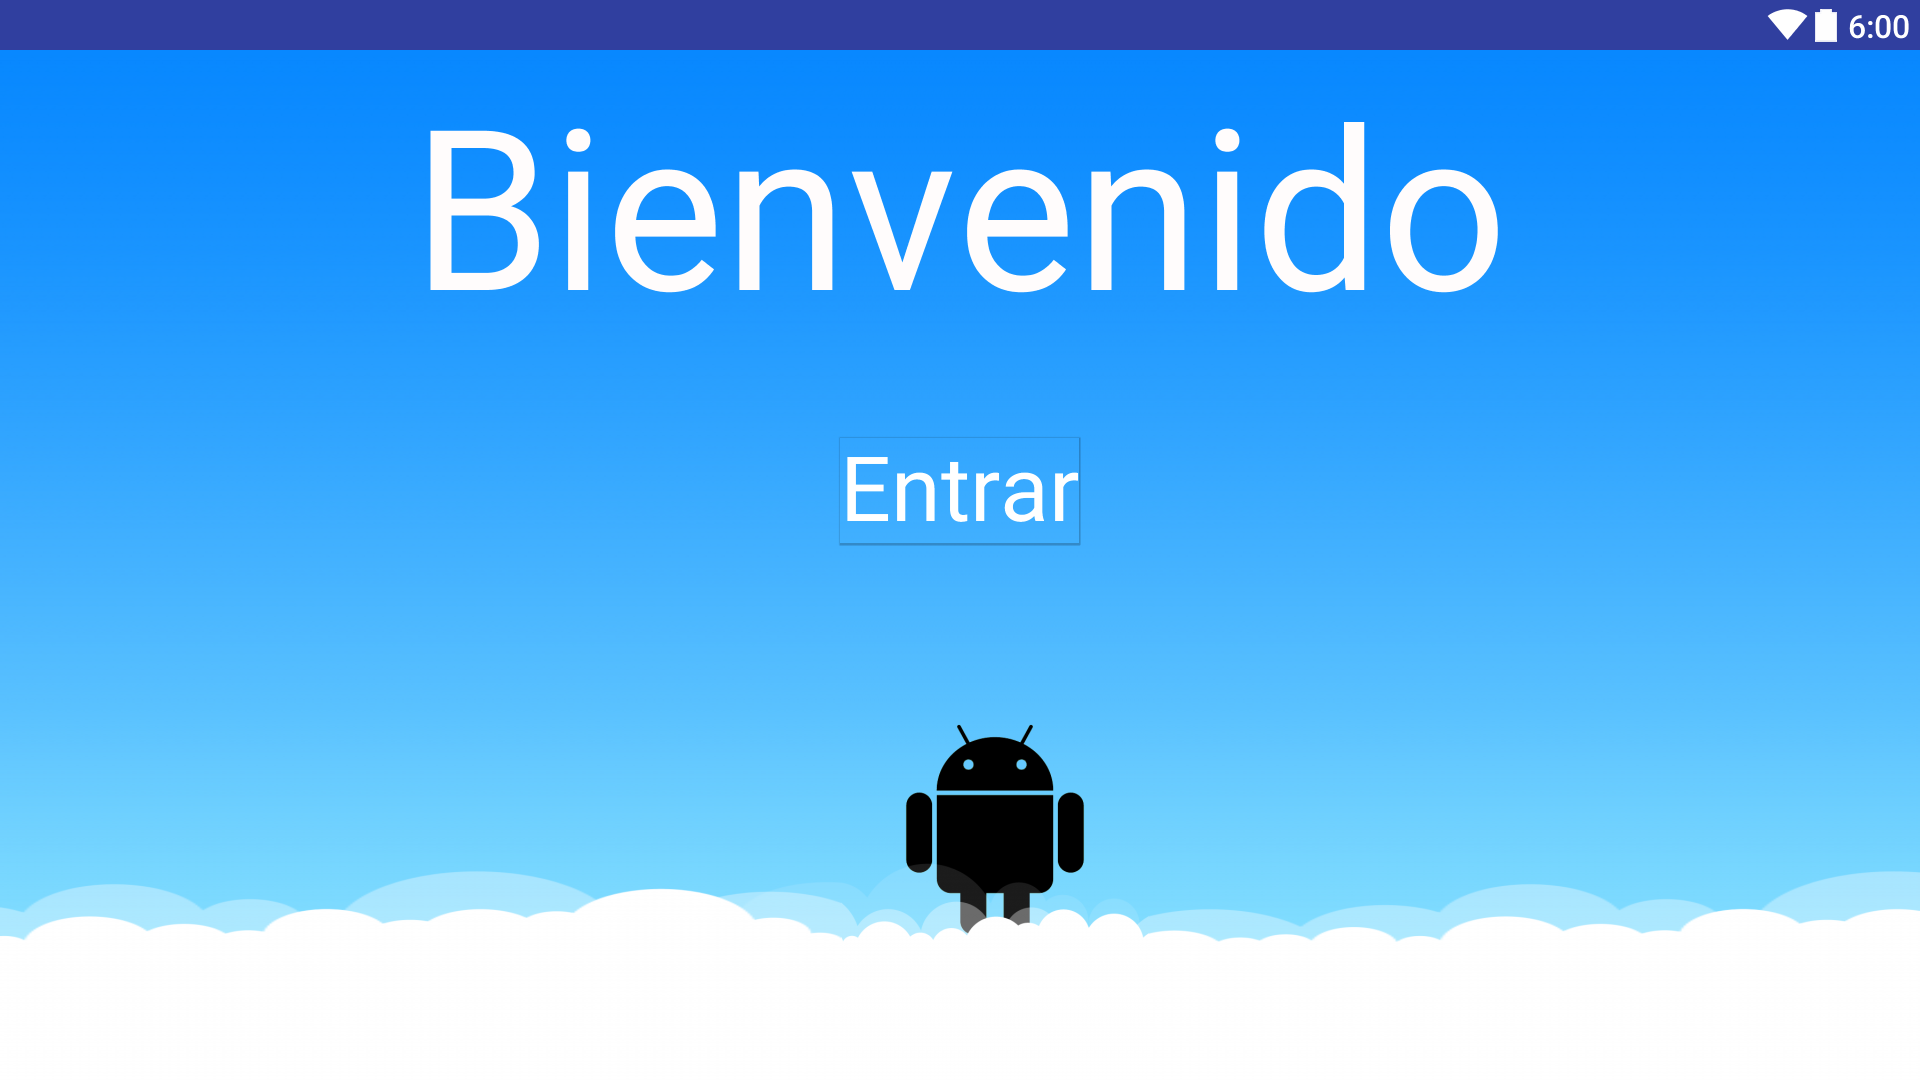
\includegraphics[scale=.2]{layout-2016-04-17-esp_TV.png} 

\end{center}

\newpage

\noindent \textbf{c) Imagen para fondo y muestra de nine-patch}\\

$\alpha$. Original

\begin{center}


\includegraphics[scale=.23]{Marcianito.png} 

\end{center}

$\beta$. 9 Patch

\begin{center}

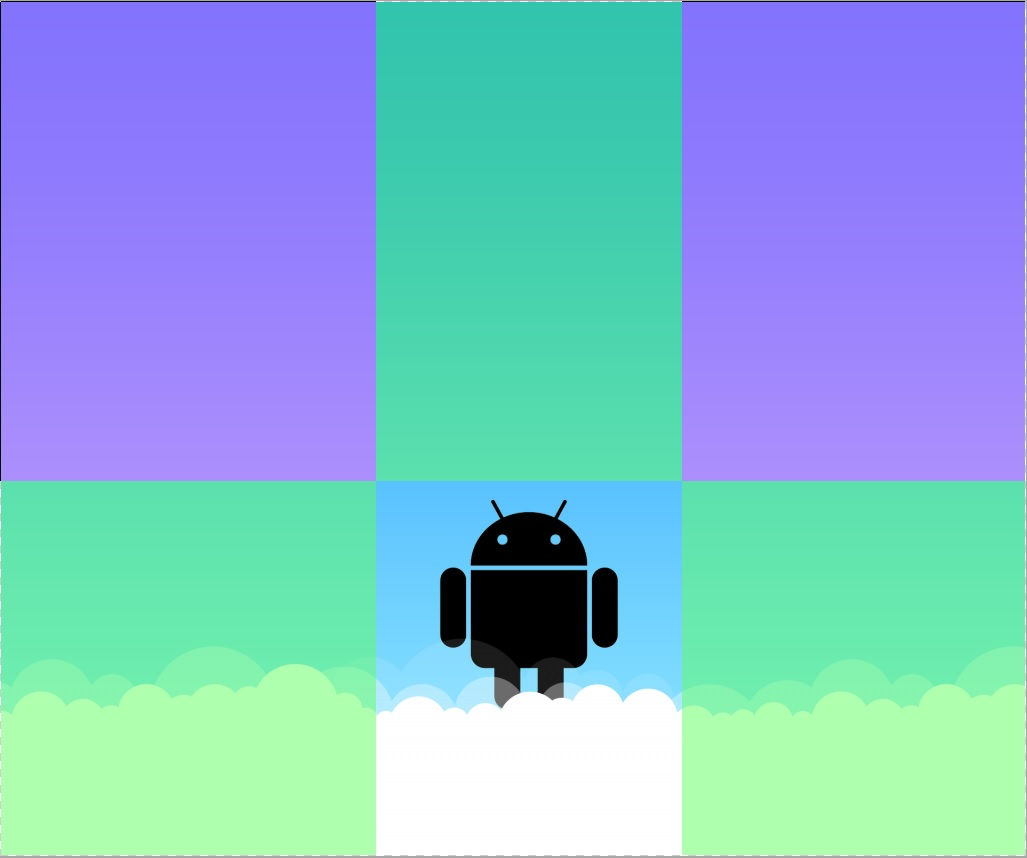
\includegraphics[scale=.3]{9patch.jpg} 

\end{center}

\end{document}